\documentclass[a4paper, 10pt]{article}

\usepackage[utf8]{inputenc}
\usepackage[margin=2.5cm, top=3.5cm]{geometry}
\usepackage[spanish]{babel}
\usepackage{graphicx}
\usepackage[hidelinks]{hyperref}
\usepackage{fancyhdr}
\usepackage{lipsum} 
\usepackage{caption}
\usepackage{xcolor}
\usepackage{colortbl}
\usepackage{float}
\usepackage{array}

% Variables
\newcommand{\logoPortada}{images/logo_uni.png}


\pagestyle{fancy}

\fancyhead[L]{\leftmark}    
\fancyhead[C]{}             
\fancyhead[R]{\textcolor{red}{\thepage}}
\fancyfoot{} 



\begin{document}

% -----------------------------------------PORTADA-------------------------------------------------------------
    \begin{titlepage}
        \centering
        \includegraphics[width=0.2\textwidth]{\logoPortada} \par\vspace{1cm}
        {\scshape\LARGE \textbf{Universidad de Sevilla}}\par\vspace{1cm}
        {\scshape\Large ESCUELA TÉCNICA SUPERIOR DE INGENIERÍA INFORMÁTICA}\par\vspace{1cm}
        GRADO EN INGENIERÍA INFORMÁTICA DEL SOFTWARE\par\vspace{1cm}
        TRABAJO FIN DE GRADO\par\vspace{1cm}
        {\huge\bfseries Desarrollo de una auditoría de ciberseguridad para PYMEs}\par\vspace{1cm}
        Realizado por:\par\vspace{0.1cm}
        {\Large\itshape Álvaro Ruiz Gutiérrez}\par\vspace{1cm}
        Dirigido por:\par\vspace{0.1cm}
        {\Large\itshape Alejandro Carrasco Muñoz}\par\vspace{1cm}
        Departamento:\par\vspace{0.1cm}
        {\Large\itshape Tecnología Electrónica}\par\vspace{1cm}
        2024/2025
    \end{titlepage}
    \clearpage
% -----------------------------------------------INDICES------------------------------------------------------------

\tableofcontents
\thispagestyle{empty}
\clearpage


\listoffigures
\thispagestyle{empty}
\clearpage


\listoftables
\thispagestyle{empty}
\clearpage


% -----------------------------------------------AGRADECIMIENTOS------------------------------------------------------------

\section*{Agradecimientos}
\thispagestyle{empty}
INTENCIONADAMENTE EN BLANCO

\clearpage

% -----------------------------------------------RESUMEN------------------------------------------------------------

\section*{Resumen}
\thispagestyle{empty}
Las pequeñas y medianas empresas (PYMEs) desempeñan un papel importante en la economía global. Sin embargo, su creciente
digitalización ha aumentado su exposición a ciberataques, debido a infraestructuras de seguridad limitadas y con recursos insuficientes para enfrentar amenazas sofisticadas. 
Este proyecto tiene como objetivo principal desarrollar un modelo de auditoría de ciberseguridad adaptado a las PYMEs, basándose en la normativa europea y nacional vigente. Para garantizar su usabilidad, se elaborará una guía accesible para usuarios sin conocimientos técnicos previos, permitiéndoles evaluar la seguridad de sus entornos digitales.
\par\vspace{0.5cm}

El proyecto se divide en dos fases principales. En la primera, se establecerá un marco teórico que explore las herramientas más comunes en auditorías de seguridad, las normativas aplicables y las metodologías más utilizadas en el ámbito de la ciberseguridad. Se examinarán los diferentes tipos de auditorías y se proporcionarán diferentes métodos para mitigar posibles riesgos. Esta fase permitirá comprender en profundidad las vulnerabilidades específicas del entorno empresarial y cómo abordarlas.
\par\vspace{0.5cm}

La segunda fase estará dedicada a la implementación práctica de la auditoría, siguiendo una 
metodología estructurada que abarcará desde el análisis del perímetro de red hasta la evaluación de la seguridad de los datos. 
Se incluirán en el diseño, pruebas en aplicaciones web, dispositivos IoT y la infraestructura interna de la empresa. 
Esta parte culminará con un caso práctico que ilustrará el proceso parcial de una auditoría de ciberseguridad en un entorno real, proporcionando una visión clara de cómo aplicar las técnicas aprendidas.
\par\vspace{0.5cm}

El objetivo principal de este estudio es facilitar la realización de auditorías de ciberseguridad en PYMEs, al tiempo que se fomenta la adopción de buenas prácticas en el ámbito de la seguridad informática. Finalmente, se incluirá un informe profesional que documente de forma detallada tanto el desarrollo del proceso de auditoría como los resultados obtenidos, proporcionando así una visión clara y estructurada del estado de ciberseguridad de la organización evaluada.

\par\vspace{0.5cm}
\textbf{Palabras clave:} ciberseguridad, auditoría, PYMEs, vulnerabilidades, normativas, metodologías, buenas prácticas.
\clearpage

% -----------------------------------------------ABSTRACT------------------------------------------------------------

\section*{Abstract}
\thispagestyle{empty}
Small and medium-sized enterprises (SMEs) play a crucial role in the global economy. However, their increasing digitalization has heightened their exposure to cyberattacks, due to limited security infrastructures and insufficient resources to counter sophisticated threats.
The main objective of this project is to develop a cybersecurity audit model tailored to SMEs, based on current European and national regulations. To ensure usability, an accessible guide will be created for users with no prior technical knowledge, enabling them to assess the security of their digital environments.
\par\vspace{0.5cm}

The project is divided into two main phases. In the first phase, a theoretical framework will be established, exploring the most common tools used in security audits, the applicable regulations, and the most widely used methodologies in the field of cybersecurity. Different types of audits will be examined, and various methods will be provided to mitigate potential risks. This phase will offer a deep understanding of the specific vulnerabilities within business environments and how to address them.
\par\vspace{0.5cm}

The second phase will focus on the practical implementation of the audit, following a structured methodology that covers everything from network perimeter analysis to data security assessment.
The design will include testing in web applications, IoT devices, and the company's internal infrastructure.
This phase will culminate in a practical case study illustrating the partial process of a cybersecurity audit in a real-world environment, offering a clear view of how to apply the techniques learned.
\par\vspace{0.5cm}

The main goal of this study is to facilitate the execution of cybersecurity audits in SMEs while promoting the adoption of best practices in the field of information security. Finally, a professional report will be included, documenting in detail both the audit process and the results obtained, thus providing a clear and structured overview of the cybersecurity status of the evaluated organization.
\par\vspace{0.5cm}
\textbf{Keywords:} cybersecurity, audit, SMEs, vulnerabilities, regulations, methodologies, best practices.
\clearpage



% -----------------------------------------------INTRODUCCION------------------------------------------------------------
\section{Introducción}
En el mundo digital actual, la ciberseguridad ya no es una opción, sino una necesidad. Las pequeñas y medianas empresas (PYMEs), pilares fundamentales de la economía global, se encuentran entre los objetivos más vulnerables frente a ciberataques. A pesar de su importancia económica, 
muchas de estas empresas subestiman su exposición a amenazas digitales, creyendo erróneamente que su tamaño las hace pasar desapercibidas para los ciberdelincuentes. Sin embargo, esta percepción es un error crítico, ya que la limitada infraestructura de seguridad de las 
PYMEs las convierte en blancos fáciles. 
\par\vspace{0.5cm}

Un claro ejemplo de la creciente amenaza cibernética es el ataque sufrido por el portal de afiliación del sindicato Comisiones Obreras (CCOO) en diciembre de 2023 \cite{farlopa}. El atacante explotó una vulnerabilidad en el formulario de afiliación, accediendo a la configuración interna del sitio web. Esta brecha permitió la subida de un archivo malicioso que otorgó control total sobre el sistema, facilitando el acceso a información sensible, incluyendo contraseñas sin la protección adecuada. Como resultado, el atacante alteró la página de inicio de aproximadamente 50 subdominios de ccoo.es, demostrando la facilidad con la que se puede comprometer la seguridad digital de una organización.
\par\vspace{0.5cm}

Este incidente subraya la necesidad de fortalecer la ciberseguridad en organizaciones de todos los tamaños. Las PYMEs, en particular, son especialmente susceptibles debido a la escasez de recursos y, en muchos casos, a una falta de concienciación sobre las amenazas digitales. 
La creciente digitalización y la dependencia de sistemas conectados a la red han ampliado la superficie de ataque, exponiendo a estas organizaciones a riesgos significativos.
\par\vspace{0.5cm}

En este contexto, es crucial que las PYMEs adopten medidas proactivas para proteger sus activos digitales. Este trabajo propone una guía práctica para la realización de auditorías de ciberseguridad, con el objetivo de identificar vulnerabilidades, evaluar riesgos y establecer 
estrategias de mitigación efectivas. A través de esta guía, se busca que las PYMEs fortalezcan su seguridad informática y enfrenten con mayor confianza los desafíos del entorno digital actual.

\clearpage



\subsection{Objetivos}

El objetivo principal de este trabajo es dise\~nar un modelo de auditor\'ia de ciberseguridad  espec\'ifico para PYMEs, que sea f\'acil de implementar por personas sin conocimientos t\'ecnicos avanzados. Los objetivos espec\'ificos incluyen:

\begin{itemize}
    \item Establecer un marco te\'orico que contemple las herramientas, t\'ecnicas y normativas actuales en ciberseguridad.
    \item Proponer una metodolog\'ia de auditor\'ia completa y estructurada.
    \item Desarrollar un caso pr\'actico en una PYME real para validar la metodolog\'ia propuesta.
    \item Redactar un informe detallado que incluya el an\'alisis de riesgos, vulnerabilidades detectadas y recomendaciones de mejora.
    \item Elaborar una guía clara y comprensible, diseñada específicamente para ser utilizada por personas sin conocimientos técnicos previos.
\end{itemize}

\subsection{Alcance}

El alcance está diseñado para cubrir todos los aspectos necesarios para realizar una auditoría de ciberseguridad efectiva en PYMEs, basándose en estándares y metodologías reconocidas internacionalmente.

\begin{enumerate}
    \item \textbf{Marco teórico:} Se explorarán las herramientas más utilizadas en auditorías de ciberseguridad, las normativas relevantes tanto a nivel nacional como europeo, los distintos tipos de auditoría existentes y las recomendaciones de organizaciones como OWASP, SANS y OSSTM.
    
    \item \textbf{Requisitos previos:} Se detallarán los conocimientos, habilidades y recursos técnicos necesarios para realizar auditorías efectivas, incluyendo la configuración de entornos de prueba y el uso de herramientas especializadas.
        
    \item \textbf{Propuesta de metodología:} Se desarrollará una metodología estructurada que incluirá el análisis exhaustivo de todos los aspectos a evaluar en una auditoria de ciberseguridad completa. Esta abarcará el perímetro de red, la seguridad inalámbrica, la identificación de vulnerabilidades, pruebas sobre aplicaciones web, evaluación de la infraestructura interna y análisis de seguridad en endpoints y sistemas de almacenamiento de datos.
    
    \item \textbf{Caso práctico:} Se implementará un caso práctico que aplicará la metodología propuesta de manera parcial en un entorno real, permitiendo ilustrar de manera tangible el proceso completo de una auditoría de ciberseguridad.
    
    \item \textbf{Informe final:} Elaboración de un documento que refleje el estado actual de la ciberseguridad en la empresa auditada y las recomendaciones pertinentes.
\end{enumerate}


\subsection{Motivación}
La creciente digitalización ha expuesto a las Pequeñas y Medianas Empresas (PYMEs) a una variedad de ciberamenazas que, de no ser gestionadas adecuadamente, 
pueden poner en riesgo la continuidad de sus operaciones. A diferencia de las grandes corporaciones, las PYMEs suelen carecer de los recursos humanos y financieros 
necesarios para implementar medidas robustas de ciberseguridad, lo que las convierte en un fácil objetivo para los ciberdelincuentes.
\par\vspace{0.5cm}
El aumento en el volumen de software malicioso, que supera los 450.000 nuevos programas diarios \cite{avtest}, y el hecho de que el 70 
por ciento de los ciberataques en la Península Ibérica afectan a PYMEs, subrayan la urgencia de desarrollar herramientas accesibles y eficaces para proteger a estas organizaciones. 
Este proyecto surge como respuesta a esa necesidad, proporcionando una guía práctica que permite a cualquier persona, independientemente de su nivel técnico, llevar a cabo una auditoría 
básica de ciberseguridad.
\par\vspace{0.5cm}
Además, una de las principales motivaciones personales que ha impulsado la realización de este trabajo es mi interés en formarme profesionalmente como pentester. 
Este proyecto representa un primer paso en ese camino, permitiéndome aplicar conocimientos teóricos y prácticos en un entorno real. Al mismo tiempo, me gustaría que esta guía 
pudiera servir como punto de partida para otros estudiantes en prácticas o personas con poca experiencia que deseen introducirse en el ámbito de la ciberseguridad. 
De este modo, no solo se contribuye a la protección de las PYMEs, sino también al desarrollo de nuevos profesionales en el sector.
\par\vspace{0.5cm}


\subsection{Requisitos formales}
Una vez dado un contexto general del trabajo, nos centraremos en describir que requisitos son necesarios para la redacción
 del documento.
\subsubsection{Documentación e información}
\begin{itemize}
    \item Los documentos pueden ser extraídos de \textit{Google Scholar} para su posterior citación, recomendando documentos no más antiguos de 3 o 4 años para asegurar la vigencia de la información.
    \item Se citarán en el documento en formato APA todos los documentos de los que se ha extraído información.
    \item Deben contener información relevante y actualizada sobre ciberseguridad en PYMEs, incluyendo normativas, estándares, herramientas y técnicas de auditoría.
\end{itemize}

\subsubsection{Normativas y certificaciones}
\begin{itemize}
    \item Deben ser oficiales y de libre acceso, proporcionadas por organismos reguladores tanto de ámbito europeo como internacional.
\end{itemize}

\subsubsection{Propuesta de metodología de la auditoría}
\begin{itemize}
    \item Debe atender a los requerimientos de ciberseguridad descritos en la documentación oficial.
    \item Describir las implementaciones de hardware y software necesarias para proteger los sistemas.
\end{itemize}

\subsubsection{Sobre el caso práctico}
\begin{itemize}
    \item Descripción del sistema auditado, incluyendo modelo y vulnerabilidades.
    \item Aplicación de la metodología de ciberseguridad en la PYME seleccionada.
    \item Detalle de las pruebas realizadas y la obtención de información sobre riesgos, amenazas y vulnerabilidades.
\end{itemize}


\subsection{Estructura del documento}

El documento está organizado en once capítulos que abordan de manera integral todos los aspectos necesarios para realizar una auditoría de ciberseguridad en PYMEs:

\begin{itemize}
    \item \textbf{Agradecimientos:} Reconocimiento a las personas y entidades que han contribuido al desarrollo de este trabajo.
    
    \item \textbf{Resumen:} Síntesis del contenido, objetivos y resultados del trabajo.
    
    \item \textbf{Introducción:} Presentación del contexto de la ciberseguridad en PYMEs, objetivos, alcance, motivación, requisitos formales para el desarrollo del proyecto y estructura del documento.
    
    \item \textbf{Planificación:} Descripción de la organización del trabajo, incluyendo cronograma, recursos utilizados, costes y fases del proyecto.
    
    \item \textbf{Marco Teórico (Estado del arte):} Análisis de normativas nacionales y europeas aplicables, estándares, herramientas de pentesting y técnicas relevantes en el ámbito de la ciberseguridad para PYMEs.
    
    \item \textbf{Requisitos:} Definición de los requisitos técnicos, necesarios para llevar a cabo una auditoría de seguridad.
    
    \item \textbf{Modelo de auditoría:} Propuesta de un modelo de auditoría dividido en diseño, metodología y fases específicas.
    
    \item \textbf{Caso Práctico:} Implementación de la auditoría en un entorno real de una PYME, aplicando las herramientas y técnicas descritas.
    
    \item \textbf{Resultados:} Presentación y análisis de los resultados obtenidos en el caso práctico.
    
    \item \textbf{Conclusión:} Reflexión sobre los hallazgos, lecciones aprendidas y posibles trabajos futuros.
    
    \item \textbf{Referencias:} Fuentes consultadas para la realización del trabajo.
    
    \item \textbf{Anexos:}  Material complementario que apoya el desarrollo del caso práctico y la comprensión de la metodología.

\end{itemize}




\clearpage

% -----------------------------------------------PLANIFICACION------------------------------------------------------------
\section{Planificación}
Este capítulo presenta la planificación detallada para el desarrollo del trabajo. Se describirán las fases y tareas específicas a desarrollar, los roles y responsabilidades de los participantes en el proyecto, así como un cronograma que permitirá visualizar el progreso del trabajo a lo largo del tiempo. Además, se identificarán los recursos necesarios para llevar a cabo el proyecto y se realizará un análisis de los costes asociados.

\subsection{Fases y lista de actividades}
\par\vspace{0.5cm}
\textbf{\large Fase 1 - Gestión del Proyecto} \vspace{0.5cm}

\begin{itemize}
    \item \textbf{1.1 Plan de Inicio}
    \begin{itemize}
        \item \textbf{1.1.1 Reunión inicial:} Primer encuentro con el tutor para explorar posibles temas de interés para el TFG.
        \item \textbf{1.1.2 Investigación preliminar:} Análisis de las diferentes opciones y selección del tema más adecuado.
        \item \textbf{1.1.3 Adjudicación TFG:} Confirmación oficial del tema y asignación del trabajo.
        \item \textbf{1.1.4 Inicio del trabajo:} Comienzo formal de la redacción y desarrollo del trabajo.
        \item \textbf{1.1.5 Investigación orientada a los objetivos:} Ampliación del conocimiento sobre el tema seleccionado.
        \item \textbf{1.1.6 Segunda reunión con el tutor:} Reunión para debatir la estructura y organización del TFG.
        \item \textbf{1.1.7 Reunión con CTO BeeHacker:} Análisis de la viabilidad del trabajo y perspectivas del sector.
        \item \textbf{1.1.8 Segunda reunión con CTO BeeHacker:} Obtención de información adicional.
        \item \textbf{1.1.9 Desarrollo de la introducción:} Definición clara de los objetivos, alcance, motivación y requisitos.
        \item \textbf{1.1.10 Revisión de la introducción:} Revisión y aprobación del plan de inicio.
    \end{itemize}

    \item \textbf{1.2 Planificación}
    \begin{itemize}
        \item \textbf{1.2.1 Definición de fases y tareas:} Establecimiento de las fases y actividades del proyecto.
        \item \textbf{1.2.2 Definición de roles y responsables:} Asignación de roles y responsabilidades del proyecto.
        \item \textbf{1.2.3 Cronograma:} Desarrollo del cronograma en MSProject.
        \item \textbf{1.2.4 Recursos:} Identificación de recursos humanos y materiales.
        \item \textbf{1.2.5 Estimación de costes:} Cálculo del presupuesto estimado.
        \item \textbf{1.2.6 Revisión de la planificación:} Revisión y aprobación de la planificación.
    \end{itemize}

    \item \textbf{1.3 Seguimiento y Control}
    \begin{itemize}
        \item \textbf{1.3.1 Corrección de la introducción:} Corrección y ajuste de la introducción.
        \item \textbf{1.3.2 Corrección de la planificación:} Corrección y ajuste de la planificación.
        \item \textbf{1.3.3 Corrección del marco teórico:} Corrección y ajuste del marco teórico.
        \item \textbf{1.3.4 Corrección del modelo de auditoría:} Corrección y ajuste del modelo de auditoría.
        \item \textbf{1.3.5 Informe y control del desempeño:} Generación de informes de seguimiento.
    \end{itemize}

    \item \textbf{1.4 Cierre}
    \begin{itemize}
        \item \textbf{1.4.1 Informe final con resultados:} Documentación final con las conclusiones.
        \item \textbf{1.4.2 Plan de mitigación de riesgos:} Propuesta de acciones correctivas.
        \item \textbf{1.4.3 Lecciones aprendidas:} Reflexión sobre los conocimientos adquiridos.
    \end{itemize}
\end{itemize}

\vspace{0.5cm}
\textbf{\large Fase 2 - Desarrollo del Producto} \vspace{0.5cm}

\begin{itemize}
    \item \textbf{2.1 Marco teórico}
    \begin{itemize}
        \item \textbf{2.1.1 Desarrollo del marco teórico:} Investigación, análisis, redacción y estructuración del marco conceptual.
        \item \textbf{2.1.2 Revisión del marco teórico:} Revisión y aprobación del marco teórico.
    \end{itemize}

    \item \textbf{2.2 Modelo de auditoría}
    \begin{itemize}
        \item \textbf{2.2.1 Diseño del modelo:} Definición de la estructura metodológica y los procedimientos a seguir.
        \item \textbf{2.2.2 Revisión del modelo:} Revisión y aprobación del modelo de auditoría.
    \end{itemize}

    \item \textbf{2.3 Caso práctico}
    \begin{itemize}
        \item \textbf{2.3.1 Desarrollo del caso práctico:} Ejecución y aplicación en la PYME.
        \item \textbf{2.3.2 Seguimiento de la práctica:} Monitorización y análisis del proceso.
    \end{itemize}
\end{itemize}

\vspace{0.5cm}
\textbf{\large Fase 3 - Revisión técnica formal} \vspace{0.5cm}

\begin{itemize}
    \item \textbf{3.1 Revisión del proyecto}
    \begin{itemize}
        \item \textbf{3.1.1} Análisis completo del trabajo desarrollado y correcciones necesarias.
    \end{itemize}
\end{itemize}

\vspace{0.5cm}
\textbf{\large Fase 4 - Presentación} \vspace{0.5cm}

\begin{itemize}
    \item \textbf{4.1 Presentación del proyecto}
    \begin{itemize}
        \item \textbf{4.1.1} Exposición y defensa del trabajo realizado.
    \end{itemize}
\end{itemize}




\subsection{Roles y responsabilidades}

\begin{table}[H]
    \centering
    \caption{Distribución de roles y responsabilidades en el proyecto}
    \begin{tabular}{|c|c|}

        \hline
        \textbf{Rol} & \textbf{Responsabilidad} \\
        \hline
        Analista/Desarrollador (Alumno) & Planificación y redacción del documento \\
        \hline
        Analista/Desarrollador (Alumno) & Investigación y análisis de ciberseguridad en PYMEs \\
        \hline
        Analista/Desarrollador (Alumno) & Desarrollo del marco teórico \\
        \hline
        Analista/Desarrollador (Alumno) & Agrupación y redacción de requisitos previos para auditoría \\
        \hline
        Analista/Desarrollador (Alumno) & Identificación y documentación de normativas aplicables \\
        \hline
        Analista/Desarrollador (Alumno) & Creación de plan de auditoría propio \\
        \hline
        Analista/Desarrollador (Alumno) & Diseño de la metodología de auditoría \\
        \hline
        Analista/Desarrollador (Alumno) & Implementación práctica de la auditoría \\
        \hline
        Analista/Desarrollador (Alumno) & Ejecución del caso práctico \\
        \hline
        Analista/Desarrollador (Alumno) & Análisis de resultados y redacción del informe final \\
        \hline
        Jefe de proyecto (Tutor) & Asesoramiento en la selección del tema y enfoque del proyecto \\
        \hline
        Jefe de proyecto (Tutor) & Orientación y supervisión del trabajo del alumno \\
        \hline
        Jefe de proyecto (Tutor) & Organizar el desarrollo del caso práctico \\
        \hline
        Jefe de proyecto (Tutor) & Correcciones y evaluación del proyecto \\
        \hline
        Jefe de equipo (CTO de BeeHacker) & Proporcionar información técnica relevante y feedback \\
        \hline
        Jefe de equipo (CTO de BeeHacker) & Validación de la metodología y resultados del caso práctico \\
        \hline

    \end{tabular}
    \begin{flushleft}\centering
        \footnotesize \textbf{Fuente:} Elaboración propia
    \end{flushleft}    
    \label{tab:distribucion_roles}
\end{table}



\subsection{Cronograma}
ANALISIS FINAL CON EL MSProject

\subsection{Recursos}

Los recursos necesarios para el desarrollo de la auditoría de ciberseguridad se dividen en tres categorías principales: recursos humanos, materiales y costos asociados. A continuación, se detallan cada uno de ellos.

\subsubsection{Recursos Humanos}

En virtud del documento oficial de la Agencia Digital de Andalucía \cite{agencia_digital}, se establecen los costes por hora de los perfiles profesionales necesarios para la realización del proyecto.

\begin{table}[H]
\caption{Recursos Humanos}
\centering
\renewcommand{\arraystretch}{1.5}
\begin{tabular}{|c|c|c|}
\hline
\textbf{Recurso} & \textbf{Tipo} & \textbf{Costo por Hora}  \\ \hline
Director de Proyecto & Trabajo & 63,75 €/h  \\ \hline
Jefe de Equipo & Trabajo & 53,55 €/h  \\ \hline
Analista & Trabajo & 47,17 €/h  \\ \hline
\end{tabular}
\begin{flushleft}\centering
    \footnotesize \textbf{Fuente:} Elaboración propia
\end{flushleft}   
\label{tab:recursos_humanos}
\end{table}



\subsubsection{Recursos Materiales}
\begin{table}[H]
\caption{Recursos Materiales}
\centering
\renewcommand{\arraystretch}{1.5}
\begin{tabular}{|c|c|c|c|c|}
\hline
\textbf{Recurso} & \textbf{Tipo} & \textbf{Costo Unitario} & \textbf{Unidades} & \textbf{Costo Total}  \\ \hline
Impresora & Material & €50,00 & 1& €50,00  \\ \hline
Disco Duro Externo & Material &  €60,00 &1& €60,00  \\ \hline
Pen Drive & Material & €20,00 & 1& €20,00  \\ \hline
Ordenador & Material & €600,00 & 1& €600,00  \\ \hline
\end{tabular}
\begin{flushleft}\centering
    \footnotesize \textbf{Fuente:} Elaboración propia
\end{flushleft}   
\label{tab:recursos_materiales}
\end{table}



\subsubsection{Costos Asociados}

\begin{table}[H]
\caption{Costos Asociados}
\centering
\renewcommand{\arraystretch}{1.5}
\begin{tabular}{|c|c|c|c|}
\hline
\textbf{Recurso} & \textbf{Tipo} & \textbf{Costo Total} & \textbf{Coste Estimado}  \\ \hline
Reserva de Contingencia & Costo & Variable & 1000€  \\ \hline
Licencias Software & Costo & Variable &  100€ \\ \hline
\end{tabular}
\begin{flushleft}\centering
    \footnotesize \textbf{Fuente:} Elaboración propia
\end{flushleft}   
\label{tab:costos_asociados}
\end{table}



\subsection{Estimación de Costes}

Considerando los recursos descritos anteriormente, se prevé que el \textbf{Analista} desempeñe un total de \textbf{300 horas de trabajo}, lo que supone un coste estimado de \underline{14.151 €}.  
\par\vspace{0.3cm}

En cuanto al \textbf{Director de Proyecto}, se estima una dedicación de \textbf{20 horas} centradas en tareas de corrección, revisión y supervisión general del proyecto, lo que representa un coste de \underline{1.275 €}.  
\par\vspace{0.3cm}

Respecto al \textbf{Jefe de Equipo}, se calcula un total de \textbf{10 horas} destinadas a la asistencia técnica y apoyo en el desarrollo de la auditoría, con un coste asociado de \underline{535,50 €}.  
\par\vspace{0.3cm}

Además, es necesario considerar los \textbf{costos adicionales asociados} al proyecto, entre los que destacan una \textbf{reserva de contingencia} de \underline{1.000 €} para posibles imprevistos y el coste de las \textbf{licencias de software} necesarias, estimado en 100 €, lo que suma un total de \underline{1.100 €}.  
\par\vspace{0.3cm}

En lo que respecta a los \textbf{recursos materiales}, se ha calculado un coste global de \underline{730 €}, correspondiente a la adquisición de los elementos físicos indispensables para el desarrollo del trabajo.  
\par\vspace{0.3cm}

Este cálculo corresponde a una \textbf{duración estimada del proyecto de 4 meses}, durante los cuales se prevé que los profesionales involucrados realicen las tareas planificadas dentro de las horas estipuladas.  

\par\vspace{0.5cm}
\textbf{De esta manera, los costes totales estimados son los siguientes:}  

\begin{table}[H]
\caption{Resumen de costes del proyecto}
\centering
\renewcommand{\arraystretch}{1.5}
\begin{tabular}{|c|c|}
\hline
\textbf{Concepto} & \textbf{Monto (€)} \\ \hline
Recursos Humanos & 15.961,50 € \\ \hline
Recursos Materiales & 730 € \\ \hline
Costos Asociados & 1.100 € \\ \hline
\textbf{Total Estimado} & \underline{\textbf{17.791,50 €}} \\ \hline
\end{tabular}
\begin{flushleft}\centering
    \footnotesize \textbf{Fuente:} Elaboración propia
\end{flushleft}   
\label{tab:resumen_costes}
\end{table}



\clearpage































% -----------------------------------------------MARCO TEÓRICO------------------------------------------------------------
\section{Fundamentos básicos de Ciberseguridad para PYMEs}

El presente marco teórico tiene como objetivo fundamentar los conceptos esenciales relacionados con la ciberseguridad en el contexto de las pequeñas y medianas empresas (PYMEs), abordando los principales riesgos y amenazas a los que se enfrentan, así como los marcos normativos que regulan la protección de sistemas y datos. Se incluyen tanto normativas nacionales como europeas, junto con recomendaciones prácticas derivadas de estándares ampliamente reconocidos como OWASP Top 10, NIST u OSSTMM.

\par\vspace{0.5cm}

Además, se analizan las técnicas empleadas durante una auditoría de ciberseguridad, así como las herramientas más relevantes utilizadas en procesos de pentesting, con el objetivo de identificar vulnerabilidades y mejorar la postura de seguridad organizacional.
\par\vspace{0.5cm}

Este análisis proporciona una base sólida para el diseño e implementación de un modelo de auditoría de ciberseguridad orientado a PYMEs, permitiendo establecer un procedimiento claro y estructurado para mejorar la seguridad, identificar vulnerabilidades y mitigar riesgos.






















\subsection{Principales amenazas y riesgos para PYMEs}

La ciberseguridad representa un desafío importante para muchas pequeñas y medianas empresas españolas. Según el informe de Hiscox, cerca del 50\% de las empresas en España sufrió algún tipo de ciberataque en 2023. Las PYMEs, en particular, son cada vez más objetivo de estos ataques debido a su limitada preparación en ciberseguridad. De hecho, solo el 61\% de las empresas con menos de 250 empleados se sienten seguras de su preparación en este sector. (Hiscox, 2022) \cite{hiscox}
\par\vspace{0.5cm}

El Instituto Nacional de Ciberseguridad (INCIBE) registró en 2022 un total de 118.000 incidentes de ciberseguridad, un 9\% más que el año anterior. Una gran parte de estos incidentes afectaron a pequeñas y medianas empresas, y uno de cada tres se trató de una filtración de datos. (INCIBE, 2023) \cite{incibe2023}
\par\vspace{0.5cm}

Aunque cada vez más PYMEs aumentan sus presupuestos en ciberseguridad y colaboran con empresas especializadas, muchas todavía optan por externalizar sus servicios por falta de personal y recursos internos. Esta externalización, si bien útil, debe complementarse con una adecuada cultura interna de seguridad, especialmente mediante la formación del personal.
\par\vspace{0.5cm}

Según PwC España, el 86\% de las organizaciones considera que sus empleados carecen de una cultura de ciberseguridad adecuada, lo que pone de relieve la necesidad urgente de concienciación. (PWC, 2021) \cite{pow}
\par\vspace{0.5cm}

Entre las principales ciberamenazas que afectan a las PYMEs según Treyder (2023) se encuentran:

\begin{itemize}
    \item \textbf{Malware:}  
    El término engloba todo tipo de software malicioso diseñado para infiltrarse o dañar un sistema sin el consentimiento del usuario. Incluye virus, troyanos, spyware y especialmente ransomware, que cifra los datos del sistema y exige un rescate económico para su recuperación. Las PYMEs suelen ser víctimas de malware distribuido por correos adjuntos infectados o a través de enlaces maliciosos en páginas aparentemente legítimas. Además del daño económico, el malware puede provocar la pérdida permanente de datos, el control remoto de equipos y el espionaje corporativo.
\end{itemize}

\vspace{0.5cm}

La relevancia del malware como una de las principales ciberamenazas se refleja claramente en su evolución histórica. Tal y como muestra el informe de AV-TEST, la cantidad total de software malicioso (malware) y aplicaciones potencialmente no deseadas (PUA) ha experimentado un crecimiento exponencial en las últimas décadas, superando en 2024 los 1.500 millones de muestras registradas a nivel mundial. Este aumento constante evidencia que las amenazas digitales siguen sofisticándose y expandiéndose, afectando por igual a grandes empresas y a pequeñas organizaciones como las PYMEs.

\vspace{0.3cm}

\begin{figure}[H]
    \centering
    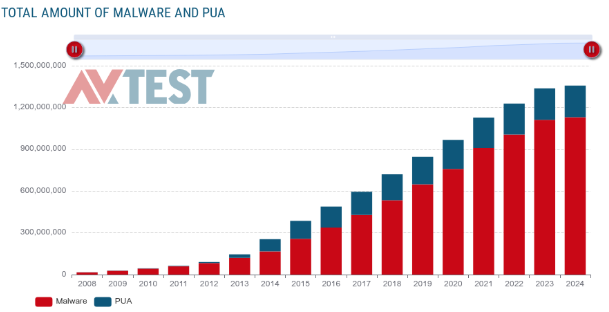
\includegraphics[width=0.95\textwidth]{images/malware.png}
    \caption{Evolución histórica de la cantidad total de malware y PUA a nivel mundial. Fuente: av-atlas.org \cite{avtest}.}
\end{figure}

\vspace{0.5cm}

Aparte del malware, existen otras amenazas igualmente relevantes para las PYMEs:

\begin{itemize}
    \item \textbf{Phishing:}  
    Consiste en técnicas de suplantación de identidad para engañar a empleados o directivos y obtener datos confidenciales, como contraseñas, credenciales bancarias o información sensible de clientes. Suele realizarse mediante correos electrónicos o mensajes falsificados que imitan a bancos, plataformas de pago o servicios tecnológicos conocidos. En las PYMEs, donde el nivel de concienciación en ciberseguridad suele ser limitado, el phishing representa una puerta de entrada frecuente a ataques más complejos, como el acceso remoto a sistemas o la instalación de malware.
    \vspace{0.3cm}

    \item \textbf{Ataques de denegación de servicio (DDoS):}  
    Este tipo de ataque busca hacer que los servidores, aplicaciones o sitios web de una empresa queden inoperativos mediante el envío masivo de peticiones falsas. Se trata de una sobrecarga intencionada de los recursos tecnológicos de la organización, que impide el funcionamiento normal de servicios clave. Aunque muchas veces se asocian a grandes empresas, las PYMEs también son objetivo, especialmente si ofrecen servicios digitales o tiendas online. Un DDoS puede paralizar las operaciones durante horas o días, con pérdidas económicas importantes y daño reputacional.
    \vspace{0.3cm}

    \item \textbf{Brechas de datos:}  
    Ocurren cuando un atacante consigue acceder sin autorización a bases de datos internas, habitualmente mediante credenciales robadas, vulnerabilidades no parcheadas o ingeniería social. Estas brechas pueden afectar a información crítica como datos de clientes, contraseñas, información financiera o planes estratégicos. Para una PYME, una brecha de datos no solo puede suponer sanciones legales —por ejemplo, si no cumple con el Reglamento General de Protección de Datos (RGPD)—, sino también pérdida de confianza por parte de clientes y socios.
    \vspace{0.3cm}

    \item \textbf{Errores de configuración:}  
    Son fallos humanos o técnicos al configurar correctamente sistemas, redes o aplicaciones. Por ejemplo, dejar puertos abiertos innecesarios, permitir contraseñas por defecto, o no establecer permisos adecuados. Estos errores abren puertas invisibles a los ciberatacantes y son especialmente comunes en entornos donde no existe un departamento de TI dedicado. La falta de mantenimiento o revisión de estas configuraciones puede convertir una infraestructura aparentemente segura en un objetivo fácil.

\end{itemize}



\par\vspace{0.5cm}
Además de los vectores de ataques mencionados anteriormente, existen ciertos \textbf{riesgos estructurales} que afectan especialmente a las PYMEs y que incrementan su vulnerabilidad frente a ciberataques:

\begin{itemize}
  \item \textbf{Falta de recursos de seguridad dedicados:} Muchas pequeñas empresas no cuentan con personal especializado en ciberseguridad (como un CISO o un técnico en protección de datos), lo que dificulta la detección y respuesta ante incidentes.
  \item \textbf{Presupuestos limitados:} La inversión en ciberseguridad suele quedar relegada frente a otras prioridades de negocio, lo que impide implementar soluciones de protección efectivas o actualizadas.
  \item \textbf{Falta de diseño seguro desde el inicio:} Al haber sido creadas por expertos en su sector y no por especialistas en tecnología, muchas PYMEs han desarrollado sus sistemas sin tener en cuenta principios de seguridad por defecto.
  \item \textbf{Ausencia de fondos de emergencia:} La falta de capacidad económica para hacer frente a pagos por rescates o pérdidas prolongadas de ingresos hace que las consecuencias de un ciberataque sean especialmente devastadoras.
  \item \textbf{Impacto operativo total ante incidentes graves:} Un ciberataque que provoque una filtración o la caída de sistemas puede detener completamente la actividad del negocio, ya que las PYMEs no suelen tener infraestructuras de respaldo.
\end{itemize}

\par\vspace{0.5cm}
Estos factores, sumados a una falsa sensación de anonimato (“somos demasiado pequeños para que nos ataquen”), aumentan considerablemente el riesgo de que las PYMEs se conviertan en blancos frecuentes y exitosos de los ciberdelincuentes. 
Implementar medidas preventivas y desarrollar una cultura de seguridad sólida resulta crucial para garantizar su continuidad. (L. Toms, 2021) \cite{toms2021}
\par\vspace{0.5cm}

Finalmente, para ilustrar en tiempo real la magnitud y frecuencia global de estos ataques y reforzar la importancia de adoptar medidas proactivas, puede consultarse el mapa interactivo proporcionado por Fortinet en el siguiente enlace: \href{https://fortiguard.fortinet.com/threat-map}{\textcolor{blue}{fortiguard.fortinet.com/threat-map}}.


\subsection{Normativas nacionales aplicables}

    En el contexto español, la legislación vigente en materia de ciberseguridad establece un conjunto de normas esenciales que las PYMEs deben tener en cuenta para garantizar la protección de sus sistemas y datos. Estas normativas buscan no solo proteger la información sensible de las organizaciones, sino también fomentar una cultura de prevención y resiliencia ante los ciberataques.
    \par\vspace{0.5cm}

    Una de las normativas más relevantes es el \textbf{Esquema Nacional de Seguridad (ENS)}, regulado por el Real Decreto 311/2022. Este marco establece los principios básicos y requisitos mínimos necesarios para una protección adecuada de la información manejada por medios electrónicos, y es de obligado cumplimiento para las entidades del sector público y recomendable para las empresas privadas. El ENS promueve un enfoque basado en riesgos y establece diferentes niveles de seguridad en función del impacto que una amenaza pueda tener sobre la organización. (Boletín Oficial del Estado, 2024). \cite{boe}
    \par\vspace{0.5cm}

    Asimismo, el \textbf{Real Decreto-ley 12/2018}, sobre seguridad de las redes y sistemas de información, incorpora al derecho español la Directiva NIS de la Unión Europea. Este decreto impone obligaciones a los operadores de servicios esenciales y proveedores de servicios digitales para garantizar un nivel adecuado de seguridad en sus operaciones, además de establecer la necesidad de notificar los incidentes de seguridad más relevantes a la autoridad competente. (Boletín Oficial del Estado, 2024). \cite{boe}
    \par\vspace{0.5cm}

    Otra normativa destacable es la \textbf{Ley Orgánica 3/2018, de Protección de Datos Personales y garantía de los derechos digitales (LOPDGDD)}, que adapta el Reglamento General de Protección de Datos (RGPD) al ordenamiento jurídico español. Esta ley establece obligaciones específicas en cuanto al tratamiento, almacenamiento y seguridad de los datos personales, lo cual es especialmente relevante en escenarios donde se procesan grandes volúmenes de datos sensibles. (Boletín Oficial del Estado, 2024). \cite{boe}
    \par\vspace{0.5cm}

    Además, organismos nacionales como el \textbf{Instituto Nacional de Ciberseguridad (INCIBE)} y el \textbf{Centro Criptológico Nacional (CCN)}  han reforzado su colaboración para coordinar acciones frente a las ciberamenazas que afectan tanto a ciudadanos como a empresas, 
    proporcionan directrices, guías técnicas y herramientas de apoyo que complementan el cumplimiento normativo, 
    especialmente adaptadas a las capacidades de las pequeñas y medianas empresas. (Escudo Digital, 2023). \cite{escudo2023}

\subsection{Normativas europeas aplicables}

    La Unión Europea ha desarrollado un marco normativo sólido para fortalecer la ciberseguridad en sus Estados miembros, afectando directamente a las PYMEs. Estas regulaciones buscan establecer un nivel común de seguridad y resiliencia operativa en el entorno digital europeo.
    \par\vspace{0.5cm}

    Una pieza clave es la \textbf{Directiva NIS2} (Directiva (UE) 2022/2555), que entró en vigor en enero de 2023. Esta directiva amplía el alcance de su predecesora, la Directiva NIS, imponiendo requisitos de seguridad más estrictos y procesos de notificación de incidentes más concretos. Se aplica a medianas y grandes empresas de sectores críticos, incluyendo energía, transporte, salud y administración pública. Las empresas deben implementar políticas de gestión de riesgos, autenticación multifactor y formación en ciberseguridad para empleados. (Cadena SER, 2024). \cite{cadena_ser}
    \par\vspace{0.5cm}

    Otra regulación relevante es el \textbf{Reglamento DORA} (Reglamento (UE) 2022/2554), que establece un marco para la resiliencia operativa digital del sector financiero. Su objetivo es garantizar que todas las entidades financieras puedan soportar, responder y recuperarse de incidentes relacionados con las TIC, asegurando la estabilidad del sistema financiero europeo. (Banco Central Europeo, 2025). \cite{bce}
    \par\vspace{0.5cm}

    Además, la propuesta de la \textbf{Ley de Ciberresiliencia} de la UE, presentada en septiembre de 2022, busca introducir requisitos horizontales obligatorios de ciberseguridad para productos con elementos digitales, garantizando que los consumidores y empresas puedan confiar en productos digitales seguros. (Comisión Europea, 2023). \cite{comision_europea}
    

    

    \subsection{Herramientas de pentesting}

    La selección de herramientas de pentesting desempeña un papel fundamental en la eficacia de las auditorías de seguridad. Identificar las herramientas adecuadas permite detectar vulnerabilidades de forma precisa y eficiente, adaptándose a distintos escenarios 
    como redes, aplicaciones web, servicios en la nube o incluso factores humanos a través de técnicas de ingeniería social. A partir de un análisis conjunto de diversas fuentes especializadas, se recopilaron las diez herramientas 
    más utilizadas y valoradas en el ámbito del pentesting. (F. Redondo \& N. Cárdenas, 2024). \cite{felipe2024}
    
    \begin{table}[H]
    \caption{Herramientas de pentesting más empleadas}
    \centering
    \begin{tabular}{|m{5cm}|m{8cm}|m{3.5cm}|}
        \hline
        \textbf{Herramienta} & \textbf{Descripción} & \textbf{Donde encontrarlas} \\
        \hline
        
\includegraphics[width=0.8cm]{images/nmap.jpeg} \textbf{Nmap} & Escáner de redes y auditor de seguridad que permite descubrir hosts, servicios y vulnerabilidades activas. & \href{https://nmap.org}{nmap.org} \\
        \hline
        
\includegraphics[width=0.8cm]{images/metasploit.jpeg} \textbf{Metasploit} & Framework completo para desarrollar, probar y ejecutar exploits en entornos controlados. & \href{https://www.metasploit.com}{metasploit.com} \\
        \hline
        
\includegraphics[width=0.7cm]{images/burp.jpeg} \textbf{Burp Suite} & Plataforma integrada para análisis de seguridad en aplicaciones web, capaz de interceptar, modificar y automatizar pruebas. & \href{https://portswigger.net/burp}{portswigger.net/burp} \\
        \hline
        
\includegraphics[width=0.85cm]{images/kali.jpeg} \textbf{Kali Linux / Parrot OS} & Sistemas operativos especializados para pentesting que incluyen múltiples herramientas de auditoría, análisis forense e ingeniería inversa. & \href{https://www.kali.org}{kali.org}, \href{https://www.parrotsec.org}{parrotsec.org} \\
        \hline
        
\includegraphics[width=0.95cm]{images/nessus.png} \textbf{Nessus} & Escáner de vulnerabilidades de red que identifica configuraciones erróneas, parches faltantes y debilidades comunes. & \href{https://www.tenable.com/products/nessus}{tenable.com/nessus} \\
        \hline
        
\includegraphics[width=0.8cm]{images/john.png} \textbf{John the Ripper} & Herramienta para craqueo de contraseñas y evaluación de su fortaleza en diferentes sistemas. & \href{https://www.openwall.com/john}{openwall.com/john} \\
        \hline
        
\includegraphics[width=0.75cm]{images/wireshark.png} \textbf{Wireshark} & Analizador de protocolos de red que permite capturar y examinar en tiempo real el tráfico que circula por una red. & \href{https://www.wireshark.org}{wireshark.org} \\
        \hline
        
\includegraphics[width=0.7cm]{images/zap.jpeg} \textbf{ZAP (Zed Attack Proxy)} & Escáner de seguridad de aplicaciones web enfocado en detectar vulnerabilidades durante el desarrollo. & \href{https://www.zaproxy.org}{zaproxy.org} \\
        \hline
        \textbf{SQLmap} & Automatiza la detección y explotación de inyecciones SQL en aplicaciones web. & \href{https://sqlmap.org}{sqlmap.org} \\
        \hline
        
\includegraphics[width=0.8cm]{images/aircrack.jpeg} \textbf{Aircrack-ng} & Conjunto de herramientas para auditar redes Wi-Fi, especializado en romper claves WEP y WPA/WPA2. & \href{https://www.aircrack-ng.org}{aircrack-ng.org} \\
        \hline
        \end{tabular}
    \begin{flushleft}\centering
        \footnotesize \textbf{Fuente:} Elaboración propia en base a (Criterios de selección de herramientas para pentesting, 2024)
    \end{flushleft}
    \end{table}



  
    
    \subsection{Técnicas utilizadas en auditorías de ciberseguridad}

    Además de contar con herramientas especializadas, una auditoría de ciberseguridad eficaz debe basarse en técnicas metodológicas contrastadas. Las técnicas descritas a continuación están ampliamente consolidadas y han sido validadas por organismos y marcos de referencia reconocidos internacionalmente, como el \textbf{PTES (Penetration Testing Execution Standard)}, el \textbf{OSSTMM (Open Source Security Testing Methodology Manual)}, el \textbf{NIST SP 800-82} para entornos industriales, y el \textbf{OWASP Top 10} en el ámbito de las aplicaciones web.
    
    \begin{itemize}
      \item \textbf{Reconocimiento (Reconnaissance):} Técnicas previas al ataque que permiten recolectar información del objetivo. Se utilizan metodologías OSINT (Open Source Intelligence), como análisis de redes sociales, WHOIS, Shodan o Google Hacking. También incluye \textit{footprinting} y \textit{fingerprinting} para identificar sistemas, servicios y versiones.
    
      \item \textbf{Escaneo y enumeración:} Se identifican puertos abiertos, servicios activos y configuraciones usando herramientas como \texttt{Nmap} o \texttt{WhatWeb}. La enumeración permite descubrir detalles específicos de servicios expuestos en la red.
    
      \item \textbf{Explotación (Exploitation):} Consiste en aprovechar vulnerabilidades detectadas para obtener acceso no autorizado a sistemas.
    
      \item \textbf{Post-explotación:} Tras comprometer un sistema, se buscan técnicas de escalado de privilegios, mantenimiento de acceso y técnicas de pivoting.
    
      \item \textbf{Análisis de vulnerabilidades:} Permite identificar y evaluar debilidades sin necesidad de explotación directa. Se emplean escáneres automáticos o revisión manual, especialmente útil en aplicaciones web, móviles o APIs.
    
      \item \textbf{Ingeniería social:} Técnica que explota el factor humano mediante engaños. Incluye phishing (correos falsos), y pretexting (identidades falsas para obtener información). Se pueden realizar simulaciones controladas para evaluar la concienciación del personal. 
    
      \item \textbf{Pentesting web:} Se prueban vulnerabilidades específicas en aplicaciones web. Para ello se suelen usar las recomendaciones de OWASP Top 10 para identificar problemas comunes en este entorno.
    
      \item \textbf{Pentesting de redes Wi-Fi:} Incluye captura de handshakes y ataques a redes WPA/WPA2/WPA3. También se realizan ataques tipo \textit{Evil Twin}, donde se simula un punto de acceso para engañar a los usuarios.
    
      \item \textbf{Ataques físicos y hardware hacking:} Cuando se tiene acceso físico a dispositivos, se pueden explotar puertos inseguros, configuraciones erróneas en BIOS, dispositivos IoT vulnerables o mediante el uso de USBs maliciosos.
    \end{itemize}
    
    
    \subsection{Buenas prácticas}
    Las buenas prácticas en el ámbito de la ciberseguridad constituyen un conjunto de acciones, políticas y medidas preventivas que buscan minimizar riesgos, proteger la información y garantizar la continuidad operativa ante posibles amenazas. En este apartado se diferenciarán dos perspectivas clave: por un lado, las buenas prácticas que una PYME debe implementar de forma interna para fortalecer su seguridad digital; y por otro, aquellas prácticas recomendadas y seguidas durante las auditorías de ciberseguridad, las cuales permiten evaluar el estado real de la infraestructura tecnológica y proponer mejoras efectivas.

    \subsubsection{Buenas prácticas en PYMES}
    
    La ciberseguridad en pequeñas y medianas empresas requiere un enfoque integral que combine herramientas, políticas, concienciación y planificación estratégica. Una única medida no es suficiente para garantizar la protección frente a las amenazas actuales. A continuación, se detallan algunas de las buenas prácticas más relevantes que una PYME debe adoptar para construir un entorno digital más seguro, según las recomendaciones de expertos (L. Toms, 2021) \cite{toms2021}:
    
    \begin{itemize}
        
        \item \textbf{Documentación de procesos y protocolos:}  
        Muchas PYMEs asignan a una sola persona la responsabilidad de la configuración y gestión de la seguridad informática. Sin embargo, esto supone un riesgo si esa persona abandona la empresa, ya que el conocimiento no queda registrado. Documentar todos los procesos, configuraciones y políticas de seguridad permite mantener la continuidad operativa, facilita auditorías internas y evita que la salida de personal clave comprometa la seguridad.
    
        \item \textbf{Contraseñas seguras y autenticación multifactorial (MFA):}  
        El uso de contraseñas débiles es una de las principales vulnerabilidades explotadas por los atacantes. Se recomienda utilizar contraseñas largas (mínimo 12 caracteres), 
        con combinación de letras, números y símbolos especiales. Además, es esencial implementar mecanismos de autenticación de doble factor (por ejemplo, mediante contraseña + huella dactilar, o código de un solo uso vía SMS), lo que añade una capa adicional de protección frente a accesos no autorizados.
    
        \item \textbf{Formación continua de los empleados:}  
        Los empleados suelen ser tanto la primera como la última línea de defensa ante ciberataques. Sin una formación adecuada, es más probable que caigan en fraudes por correo electrónico, 
        enlaces maliciosos o campañas de phishing dirigidas. Las PYMEs deben establecer programas de concienciación en ciberseguridad que incluyan formación sobre detección de amenazas, políticas de uso de dispositivos personales, buenas prácticas en navegación, y respuesta ante incidentes.
    
        \item \textbf{Enfoque de seguridad por capas (defensa en profundidad):}  
        La protección de los sistemas debe estar basada en múltiples niveles de seguridad que actúen de forma coordinada. Entre las medidas recomendadas se incluyen: 
        antivirus y antispyware actualizados, configuración adecuada del firewall, control de accesos, cifrado de los datos en tránsito y en reposo, y uso de firmas digitales para garantizar la integridad de los documentos. Esta arquitectura de defensa en profundidad mejora la resiliencia frente a ataques dirigidos o automatizados.
    
        \item \textbf{Copias de seguridad regulares y distribuidas:}  
        Las copias de seguridad son fundamentales para asegurar la recuperación de datos tras incidentes como ransomware, fallos de hardware o errores humanos. Se recomienda realizar copias frecuentes, almacenarlas en diferentes ubicaciones (local, nube o dispositivos externos), y verificar periódicamente que pueden restaurarse correctamente. Esta práctica sencilla puede marcar la diferencia entre la continuidad del negocio o la pérdida irreversible de información crítica.
    
    \end{itemize}
    
    \subsubsection{Buenas prácticas en auditorías de ciberseguridad}

    Las auditorías son procesos estructurados que permiten evaluar el estado de la seguridad informática de una organización. 
    Para que sean eficaces, deben llevarse a cabo bajo un conjunto de buenas prácticas que garanticen no solo la calidad técnica del análisis, sino también la ética profesional, 
    la trazabilidad de los hallazgos y la aplicabilidad de las recomendaciones. A continuación, se describen las principales buenas prácticas que deben seguirse durante una auditoría de ciberseguridad:
    
    \begin{itemize}
    
        \item \textbf{Definición clara del alcance:}  
        Antes de iniciar cualquier auditoría, es fundamental delimitar qué sistemas, redes, aplicaciones, ubicaciones y personas serán objeto de evaluación. Un alcance bien definido evita malentendidos, asegura que los recursos estén disponibles y permite centrar los esfuerzos en los activos más críticos.
    
        \item \textbf{Formalización mediante acuerdos previos:}  
        Toda auditoría debe comenzar con la firma de acuerdos de confidencialidad (NDA) y documentos de autorización por parte de la empresa auditada. Esto garantiza que el proceso se realice dentro del marco legal y ético, y protege tanto al auditor como a la organización.
    
        \item \textbf{Aplicación de metodologías reconocidas:}  
        Las auditorías deben basarse en estándares y marcos metodológicos ampliamente aceptados, como PTES (Penetration Testing Execution Standard), OSSTMM (Open Source Security Testing Methodology Manual), o las guías del NIST (por ejemplo, SP 800-115). Esto asegura un enfoque sistemático, riguroso y alineado con las mejores prácticas internacionales.
    
        \item \textbf{Uso controlado de herramientas especializadas:}  
        El empleo de herramientas debe realizarse de forma responsable, en entornos previamente autorizados, y con medidas que minimicen posibles interrupciones del servicio. Se recomienda documentar cada herramienta utilizada, junto con su propósito y los resultados obtenidos.
    
        \item \textbf{Documentación exhaustiva de hallazgos:}  
        Cada vulnerabilidad o debilidad detectada debe registrarse con claridad, incluyendo una descripción técnica, nivel de riesgo, posible impacto y evidencias que lo respalden. Esta documentación será esencial para la elaboración del informe final.
    
        \item \textbf{Informe técnico y ejecutivo:}  
        El resultado de la auditoría debe presentarse en dos formatos: uno técnico, dirigido al personal de sistemas, y otro ejecutivo, accesible para la dirección de la empresa. Ambos informes deben incluir un plan de acción priorizado y recomendaciones específicas y viables.
    
        \item \textbf{Propuesta de mejora continua:}  
        La auditoría no debe verse como un fin en sí misma, sino como parte de un proceso de mejora continua. Es importante que el informe incluya sugerencias para establecer controles recurrentes, políticas de seguridad y mecanismos de revisión periódica.
    
        \item \textbf{Ética profesional y confidencialidad:}  
        Durante todo el proceso, el equipo auditor debe actuar con responsabilidad, integridad y confidencialidad. Cualquier hallazgo crítico debe comunicarse de inmediato a los responsables de seguridad de la organización, sin esperar al informe final.
    
    \end{itemize}
    
 
    \clearpage
    
    
    



























































% -----------------------------------------------MODELO------------------------------------------------------------
\section{Modelo de auditoría}

El presente capítulo tiene como objetivo presentar un modelo de auditoría de ciberseguridad diseñado específicamente para las PYMES. 

\par\vspace{0.5cm}


Este modelo ha sido construido siguiendo el \textbf{roadmap de auditoría de seguridad de la empresa BeeHacker}, una guía profesional y actualizada basada en la experiencia real de entornos empresariales. La estructura modular y escalable del modelo permite adaptarlo fácilmente a los recursos y necesidades concretas de cualquier pyme, haciendo uso de herramientas tanto comerciales como de código abierto.





\subsection{Diseño}

El modelo de auditoría propuesto se basa en un enfoque estructurado por capas, abarcando todos los vectores de ataque potenciales desde el perímetro exterior hasta los datos almacenados internamente. Este diseño tiene como objetivo principal proporcionar una guía clara, práctica y completa, que permita auditar la ciberseguridad en una pyme sin necesidad de poseer conocimientos técnicos avanzados. 




Para facilitar su implementación, el modelo se presenta de forma  secuencial, asegurando así una cobertura de todos los posibles puntos débiles en la infraestructura.
\par\vspace{0.5cm}

Cada bloque está diseñada para abordar distintos ámbitos de seguridad que una pyme debe considerar prioritarios ante posibles amenazas.

\par\vspace{0.5cm}

El modelo se compone específicamente de siete grandes bloques o capas diferenciadas que permiten un análisis integral de la seguridad:

\begin{figure}[H]
    \centering
    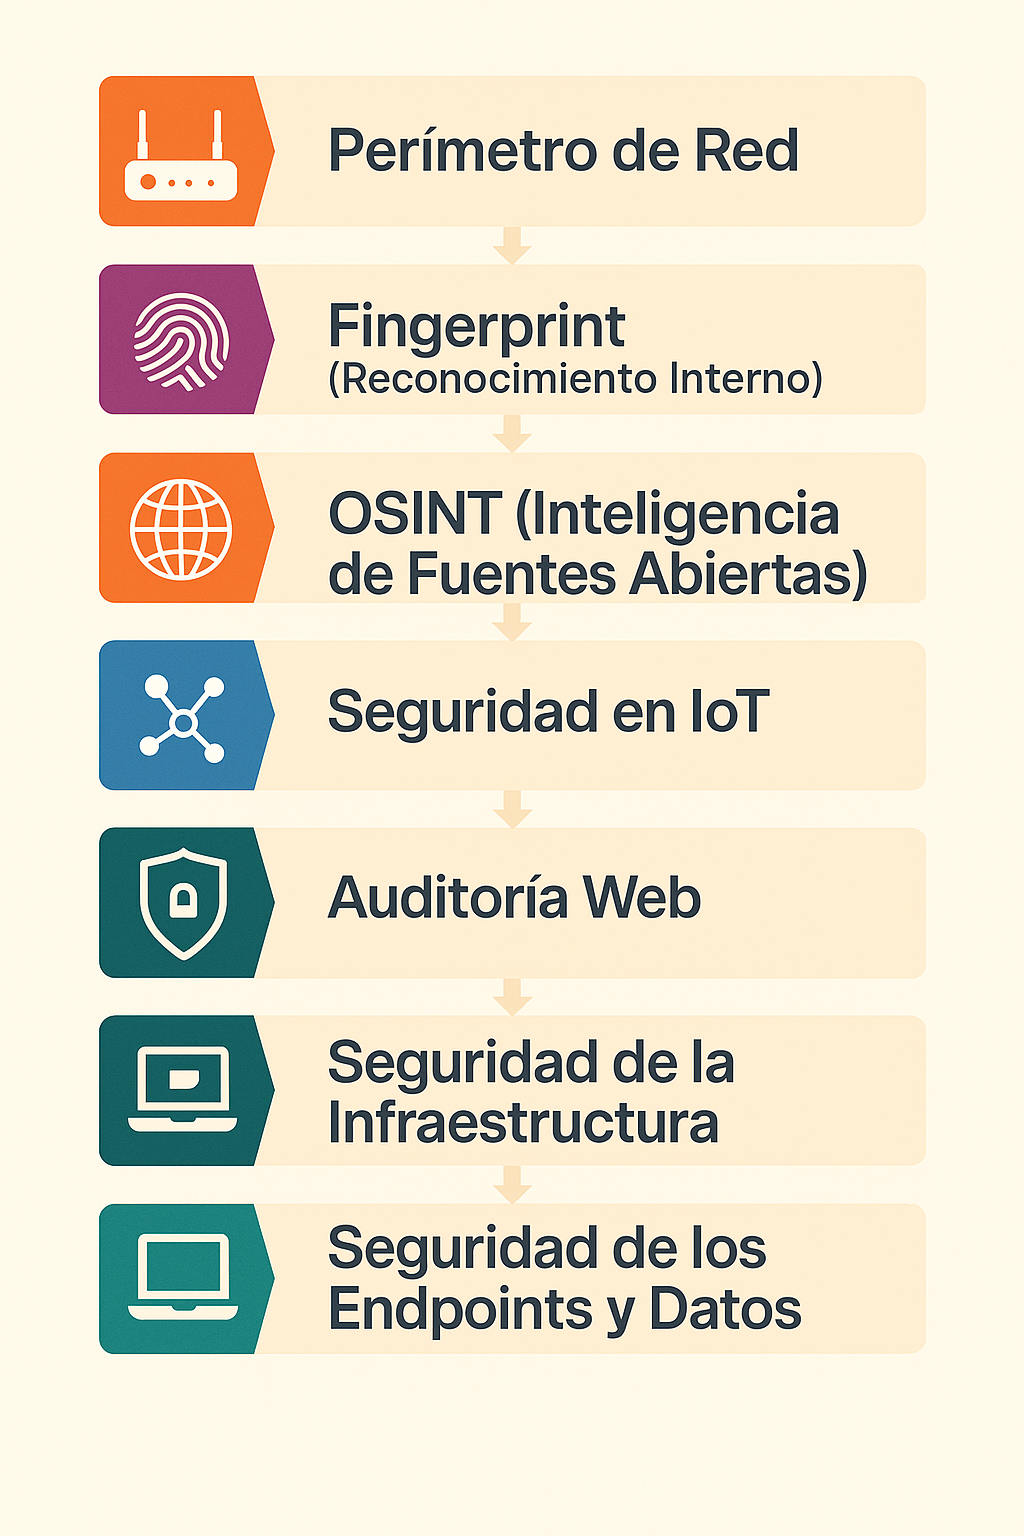
\includegraphics[width=0.45\textwidth]{images/diseno.png}
    \caption{Representación gráfica de los bloques del diseño del modelo de auditoría. Fuente: Elaboración propia}
    \label{fig:diseno_modelo_auditoria}
\end{figure}

\begin{enumerate}
\item \textbf{Perímetro de Red:} Se audita todo aquello expuesto directamente a Internet. La importancia de esta fase radica en prevenir accesos no autorizados desde el exterior. Se consideran vulnerabilidades en routers, configuraciones por defecto, firewalls mal gestionados, accesos remotos desprotegidos y redes inalámbricas sin seguridad suficiente. La auditoría abarca pruebas de acceso remoto, cifrado, filtrado de tráfico y uso de puertos abiertos.

\item \textbf{Fingerprint (Reconocimiento Interno):} Una vez superada la capa de perímetro, se simula el acceso de un atacante que ha comprometido algún sistema interno. En esta fase se identifican equipos conectados, topología de red, servicios internos, sistemas operativos y versiones. Se analiza el posible aprovechamiento de vulnerabilidades internas, uso de herramientas de enumeración, y búsqueda de servicios desactualizados o con configuraciones incorrectas.

\item \textbf{OSINT (Inteligencia de Fuentes Abiertas):} Este bloque permite identificar vectores de ataque mediante información pública sobre la empresa. Herramientas como GHDB, Shodan, Censys y Maltego se utilizan para descubrir servidores expuestos, filtraciones de credenciales, tecnologías usadas, versiones específicas y datos personales de empleados. También se evalúan técnicas de ingeniería social, como phishing o vishing.

\item \textbf{Seguridad en IoT:} Dado que muchas pymes incorporan dispositivos inteligentes como cámaras, sensores o asistentes virtuales, esta fase analiza posibles accesos no autorizados a través de estos dispositivos, los cuales suelen estar poco protegidos. Se revisa su firmware, autenticación, cifrado y su exposición en la red, así como la posibilidad de que sirvan como punto de entrada para otros ataques.

\item \textbf{Auditoría Web:} Se trata de una de las capas más críticas. Abarca tanto los servidores como las aplicaciones web y sus respectivas interfaces. Se realizan pruebas de seguridad OWASP, auditoría de formularios, análisis de sesiones, validaciones, autenticación, autorización, y pruebas automatizadas como fuzzing y spidering para descubrir rutas ocultas o vulnerables.

\item \textbf{Seguridad de Infraestructura:} Incluye todo lo relativo a la arquitectura interna: servidores, redes privadas, Active Directory, firewalls internos, IDS/IPS, políticas de red, etc. Se estudia la resistencia a técnicas de escalado de privilegios, movimiento lateral (pivoting), sniffing de tráfico y configuración segura de los distintos elementos. También se analizan los logs y sistemas de monitoreo.

\item \textbf{Seguridad de Endpoints y Datos:} Se analiza la protección de los dispositivos finales utilizados por los empleados, donde suele recaer una parte crítica de la seguridad. Se auditan políticas de contraseñas, cifrado de disco, control de dispositivos USB, protección frente a malware, uso de software legítimo, backup de información, y sistemas de almacenamiento y recuperación ante desastres.

\end{enumerate}

Cada bloque está apoyado por pruebas, herramientas y prácticas reales utilizadas en entornos profesionales, garantizando su aplicabilidad en el contexto de una pyme española.

\subsection{Propuesta de auditoría}

La propuesta consiste en ejecutar una auditoría técnica integral y realista sobre una pyme, utilizando como base el roadmap de ciberseguridad proporcionado por BeeHacker. Esta propuesta contempla los siete bloques del diseño anterior y define para cada uno una serie de actividades, herramientas y objetivos específicos, que se adaptan a los recursos y limitaciones habituales de una pyme. La auditoría se plantea en orden lógico, desde el exterior hacia el interior de la infraestructura, garantizando así la detección progresiva de riesgos.

\begin{enumerate}
\item \textbf{Análisis del Perímetro de Red:} Identificación de servicios expuestos (Nmap), comprobación de configuraciones por defecto (telnet, SSH, HTTP sin HTTPS), pruebas de red inalámbrica (Aircrack-ng, Wireshark), análisis de captivos (Bypass de portal), detección de AP falsos (Rogue AP).

\item \textbf{Fingerprinting Interno:} Escaneo de red (Netdiscover, Nmap), enumeración de servicios (SMB, RDP, FTP), análisis de versiones y vulnerabilidades (Nessus, OpenVAS), mapeo de topología (Nmap + scripts).

\item \textbf{OSINT:} GHDB para dorks avanzados, búsqueda de dispositivos en Shodan/Censys, ingeniería social (correo, LinkedIn), mapeo de dominios y subdominios (theHarvester), búsqueda de leaks (HaveIBeenPwned).

\item \textbf{Seguridad en IoT:} Escaneo de puertos y servicios, revisión de interfaces web de gestión, comprobación de firmware obsoleto, uso de exploits conocidos (CVE en dispositivos).

\item \textbf{Auditoría Web:} OWASP ZAP, Burp Suite, SQLMap, Nikto, pruebas de login, gestión de cookies, validaciones del lado cliente y servidor, búsqueda de archivos ocultos, pruebas automatizadas de fuzzing y spidering.

\item \textbf{Seguridad de Infraestructura:} Revisión de políticas en AD, prueba de escalado de privilegios (Windows/Linux), detección de usuarios con privilegios excesivos, análisis de logs, pruebas de IDS (Snort), validación de configuración de firewalls internos.

\item \textbf{Seguridad de Endpoints y Datos:} Verificación de antivirus y EDR, cifrado de disco, bloqueo de puertos físicos, revisión de backup local/remoto, gestión de contraseñas, uso de herramientas como USBDeview, VeraCrypt, Clonezilla.

\end{enumerate}

Esta propuesta se adapta a los recursos habituales de una pyme, haciendo uso de herramientas gratuitas y de código abierto siempre que sea posible, y priorizando acciones con mayor impacto y menor coste.

\subsection{Metodología de auditoría}

La auditoría se llevará a cabo mediante una metodología híbrida que combina enfoques \textbf{White Box} (con conocimiento previo de la estructura interna) y \textbf{Grey Box} (con acceso parcial), simulando escenarios realistas como los que podrían surgir en ataques internos o a través de empleados con conocimientos limitados pero con acceso legítimo.

Las fases metodológicas que se aplicarán durante la auditoría son:

\begin{enumerate}
\item \textbf{Planificación:} Definición del alcance, recursos disponibles, cronograma, responsables y objetivos específicos. Se documenta el entorno inicial y se establecen los límites éticos y técnicos de la auditoría.

\item \textbf{Reconocimiento y Enumeración:} Búsqueda de información previa con OSINT, escaneo del entorno, fingerprinting interno y externo, identificación de equipos, servicios y puertos disponibles. Se documenta todo el entorno inicial para trazar una línea base.

\item \textbf{Evaluación de Seguridad:} Ejecución práctica de las pruebas definidas en la propuesta. Se documentan vulnerabilidades, configuraciones inseguras, errores de diseño, exposición innecesaria y carencias organizativas. Se utilizan herramientas manuales y automáticas.

\item \textbf{Análisis de Riesgos:} Se evalúa la probabilidad de explotación de cada hallazgo, su impacto sobre el negocio y la posibilidad de encadenar vulnerabilidades. Se aplica una matriz de criticidad y se priorizan riesgos.

\item \textbf{Informe Final:} Se elabora un documento técnico con todos los hallazgos, acompañado de evidencias, explicación de riesgos, herramientas utilizadas, niveles de criticidad, y recomendaciones de mejora. Se incluyen propuestas técnicas y organizativas, diferenciadas por prioridad.

\end{enumerate}

El objetivo es asegurar una ejecución rigurosa, realista, replicable y proporcional a los recursos de una pyme. La metodología está diseñada para integrarse en procesos de mejora continua y cultura de seguridad progresiva.

\clearpage

% -----------------------------------------------REQUISITOS------------------------------------------------------------
\section{Requisitos}
En este capítulo se definen los requisitos esenciales para llevar a cabo una auditoría de ciberseguridad en el entorno de una PYME.

1. PC CON Linux
2. herramientas de pentesting como antenas, cactus, pen, flipper zero... 
3. herramientas de escaneo como nmap, nessus, openvas, burp suite, zap, sqlmap, nikto, etc.
4. herramientas de OSINT como shodan, censys, theharvester, maltego, etc.
5. herramientas de análisis de tráfico como wireshark, tcpdump, etc.
6. herramientas de análisis de vulnerabilidades como metasploit, bloodhound, crackmapexec, mimikatz, etc.


\subsection{Referencias y Descargas de Herramientas}

\begin{table}[H]
\centering
\begin{tabular}{|p{4cm}|p{8cm}|}
\hline
\textbf{Herramienta} & \textbf{URL de referencia / descarga} \\
\hline
Kali Linux & \url{https://www.kali.org} \\
Parrot OS & \url{https://www.parrotsec.org} \\
Nmap & \url{https://nmap.org} \\
Nessus & \url{https://www.tenable.com/products/nessus} \\
OpenVAS & \url{https://www.greenbone.net/en/} \\
Nikto & \url{https://github.com/sullo/nikto} \\
SQLMap & \url{https://sqlmap.org} \\
Burp Suite & \url{https://portswigger.net/burp} \\
OWASP ZAP & \url{https://www.zaproxy.org} \\
Shodan & \url{https://www.shodan.io} \\
Censys & \url{https://censys.io} \\
TheHarvester & \url{https://github.com/laramies/theHarvester} \\
Maltego & \url{https://www.maltego.com} \\
Wireshark & \url{https://www.wireshark.org} \\
Tcpdump & \url{https://www.tcpdump.org} \\
Metasploit & \url{https://www.metasploit.com} \\
BloodHound & \url{https://github.com/BloodHoundAD/BloodHound} \\
CrackMapExec & \url{https://github.com/Porchetta-Industries/CrackMapExec} \\
Mimikatz & \url{https://github.com/gentilkiwi/mimikatz} \\
Flipper Zero & \url{https://flipperzero.one} \\
USB Rubber Ducky & \url{https://shop.hak5.org/products/usb-rubber-ducky-deluxe} \\
Cactus WHID & \url{https://github.com/spacehuhntech/WHID-Injector} \\
\hline
\end{tabular}
\caption{Listado de herramientas utilizadas en auditorías de ciberseguridad y sus referencias oficiales}
\end{table}


\clearpage







% -----------------------------------------------CASO PRÁCTICO------------------------------------------------------------
\section{Caso Práctico}

En este capítulo se presenta el caso práctico de la auditoría de cibersegurida, en colaboración con el equipo profesional de \textbf{BeeHacker}. Esta colaboración ha permitido aplicar un modelo de auditoría actualizado y adaptado específicamente al entorno de una pyme industrial, siguiendo la metodología detallada en el capítulo anterior.


\subsection{Implementación de la auditoría}


\clearpage

% -----------------------------------------------RESULTADOS------------------------------------------------------------
\section{Resultados}



\clearpage

% -----------------------------------------------CONCLUSIONES O DISCUSIONES------------------------------------------------------------
\section{Discusión de resultados o conclusiones}



\clearpage

% -----------------------------------------------REFERENCIAS------------------------------------------------------------
%Poner bien las referencias en APA, en word puedo crear las bibliografias ya sean de entrevistas a empresas, webs, articulos... Se citan  \cite{farlopa} en el código para un ajuste final de la bibliografía.
\begin{thebibliography}{20}
    
    \bibitem{farlopa}
    DefSec. (s.f.). \textit{Mariscada virtual en el servidor de CCOO}. Recuperado el 08 de febrero de 2025, de \url{https://defsec.noblogs.org/mariscada-virtual-en-el-servidor-de-ccoo/}
    
    \bibitem{avtest}
    AV-TEST. (s.f.). \textit{AV-Atlas Malware Portal}. Recuperado el 10 de enero de 2025, de \url{https://portal.av-atlas.org/malware}
    
    \bibitem{agencia_digital} 
    Agencia Digital de Andalucía. (2024). \textit{Documento de transparencia sobre costes laborales en perfiles TIC}. Encontrado el 13 de febrero de 2025, de \url{https://ws040.juntadeandalucia.es/webconsejos/cgobierno/transparencia/240730/documentos/30Expediente.pdf}
    
    \bibitem{vuln}
    Morales-López \& Taipe-Yanez \& Pallo-Tulmo, (2024) \textit{Estrategias de Auditoría en ciberseguridad y su importancia en las empresas una revisión bibliográfica} Encontrado el 07 de abril de 2025 de \url{https://www.investigarmqr.com/ojs/index.php/mqr/article/view/1436/4849}

    \bibitem{boe}
    Boletín Oficial del Estado. (2024). Código Electrónico de Ciberseguridad. el 08 de abril de 2025 Recuperado de: \url{https://www.boe.es/biblioteca_juridica/codigos/codigo.php?id=173}

    \bibitem{cadena_ser}
    Cadena SER. (2024). ¿Qué cambia la directiva de la UE que mejora la ciberseguridad y ya aplican los Estados?. el 08 de abril de 2025 Recuperado de: \url{https://cadenaser.com/cmadrid/2024/10/22/que-cambia-la-directiva-de-la-ue-que-mejora-la-ciberseguridad-y-ya-aplican-los-estados-ser-madrid-sur/}

    \bibitem{bce}
    Banco Central Europeo. (2025). Decisiones adoptadas por el Consejo de Gobierno del BCE. el 08 de abril de 2025 Recuperado de: \url{https://www.ecb.europa.eu/press/govcdec/otherdec/2025/html/ecb.gc250131~d2c6d582b0.es.html}

    \bibitem{comision_europea}
    Comisión Europea. (2023). Una Europa Adaptada a la Era Digital. Recuperado de:el 08 de abril de 2025  \url{https://commission.europa.eu/strategy-and-policy/priorities-2019-2024/europe-fit-digital-age_es}

    \bibitem{escudo2023}
    Escudo Digital. (2023). INCIBE, CNI y CCN se reúnen para impulsar su coordinación en ciberseguridad. Recuperado de: \url{https://www.escudodigital.com/ciberseguridad/incibe-cni-ccn-se-reunen-impulsar-su-coordinacion-en-ciberseguridad_54930_102.html}

    \bibitem{felipe2024}
    Felipe Redondo, A. M., \& Núñez Cárdenas, F. J. (2024). \textit{Criterios de selección de herramientas para pentesting}. Ciencia Huasteca Boletín Científico de la Escuela Superior de Huejutla, 12(24), 31-35. Recuperado de \url{https://repository.uaeh.edu.mx/revistas/index.php/huejutla/article/view/12763/11251}
    
    \bibitem{hiscox}
    Hiscox (2022). \textit{ 44\% de las pymes españolas sufrió al menos un ciberataque durante 2021} Recuperado de \url{https://www.hiscox.es/el-44-de-las-pymes-espanolas-sufrio-al-menos-un-ciberataque-durante-2021}

    \bibitem{incibe2023}
    INCIBE (2023). \textit{INCIBE gestionó más de 118.000 incidentes de ciberseguridad durante 2022, un 9\% más que en 202} Recuperado de \url{https://www.incibe.es/incibe/sala-de-prensa/incibe-gestiono-mas-115000-incidentes-ciberseguridad-durante-2022-9-mas}

    \bibitem{pow}
    POW (2021). \textit{El 86\% de las compañías españolas carecen de una cultura de ciberseguridad entre los empleados} Recuperado de \url{https://www.pwc.es/es/sala-prensa/notas-prensa/2021/companias-espanolas-cultura-ciberseguridad-empleados.html}

    \bibitem{toms2021}
    Toms, L. (2021). \textit{5 riesgos de seguridad para las PYMEs que se deben tener en cuenta} Recuperado de \url{https://www.globalsign.com/es/blog/top-5-pequena-empresa-grandes-riesgos-5-riesgos-de-seguridad-para-las-pymes-que-se-deben-tener-en-cuenta}
    
\end{thebibliography}


\clearpage











\end{document}